\chapter{B spline curse}

\section{B Spline History}

\section{B Spline curve' definition and its properties}

\section{de Boor alorgithm}



\section{The deviation of B spline curve}

\section{B spline curse and it's deviation}

The power k to B spline curve is very important. It's decide the deviation of B spline curve. And the deviation of B spline curve is also decide by the knot vector. So we need to know the deviation of B spline curve.\\

\section{B spline and Bezier curve}

Using k power to B spline $s(u)=\sum\limits_{i=0}^{n} N_{i}^{k}(u)$ and Bezier curve $s(u)=\sum\limits_{i=0}^{n} B_{i}^{n}(u)$, we can get the relationship between B spline and Bezier curve. The curve is equaled between B spline and Bezier \\

\begin{definition}[]
	The control poind of terminate B spline curve is $s(u) = \sum_{i=0}^{k}d_i N_{i}^{k}(u)$ and the control poind of terminate Bezier curve is $P(t) = \sum\limits_{i=0}^{k}b_i B_{i}^{k}(t) $.Then we can get the relationship between B spline and Bezier curve.\[
		[b_0,b_1,...,b_k]^T = M[d_0,d_1,...,d_k]^T
	\]
\end{definition}



\newpage


\subsection{de Rham alorgithm}
de Rham alorgithm can deviate a series of $S_k$‘limitations is that $C(S_0,T) = \lim\limits_{k\rightarrow \inf}S_k$


\begin{figure}
	\begin{center}
		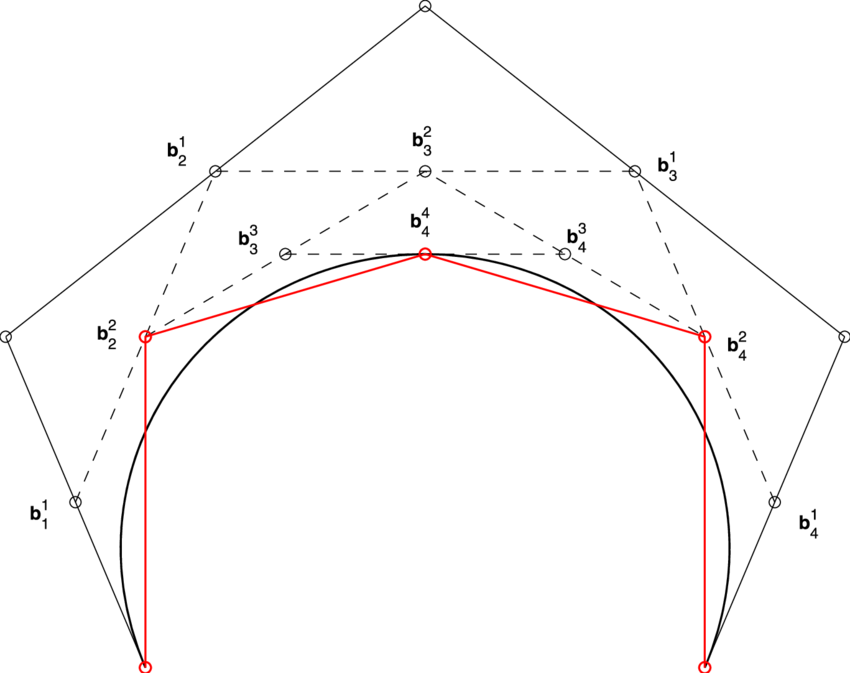
\includegraphics[scale=1]{~/Desktop/Documents/tex/CAGD/img/1.png}
	\end{center}
	\caption{}\label{fig:}
\end{figure}

\subsubsection{de Rham Curce Continuity}

\begin{property}[Continuity]
	when $0<\lambda _{i,k},\mu_{i,k},\lambda_{i,k}+\mu_{i,k}<1$,de Rham curves $S_k$ is continuted。Assum that $<p_{i-1}^{k}p_{i}^{k},p_{i}^{k}p_{i=1}^{k}>$
\end{property}

\begin{property}[Fractional dimension]
	\begin{enumerate}
		\item F has unumberable many structure
		\item F is not formular, but it's can be described by computer
		\item Different F has the same as topological dimension
		\item F's fractional dimension is larger than it's topological dimension
	\end{enumerate}
\end{property}
